
\documentclass[a4paper]{book}
\usepackage[spanish,es-tabla]{babel}
\usepackage[utf8]{inputenc}
\usepackage{graphicx}
\usepackage{multirow}
\usepackage{subfigure}
\usepackage{capt-of}
\usepackage{multirow,array}
\usepackage{float}
\usepackage{hieroglf}
\usepackage{pdfpages}

\title{Manual de usuario del robot Justina}
\author{Laboratorio de Biorobótica}
\begin{document}
\maketitle

\tableofcontents

%Inicio de la introducción
\chapter{Introducción}
En la figura \ref{fig:introduction:Justina} se muestra el robot Justina el cual es un robot de

%Figura 1.1 de Justina
\begin{figure}
\centering
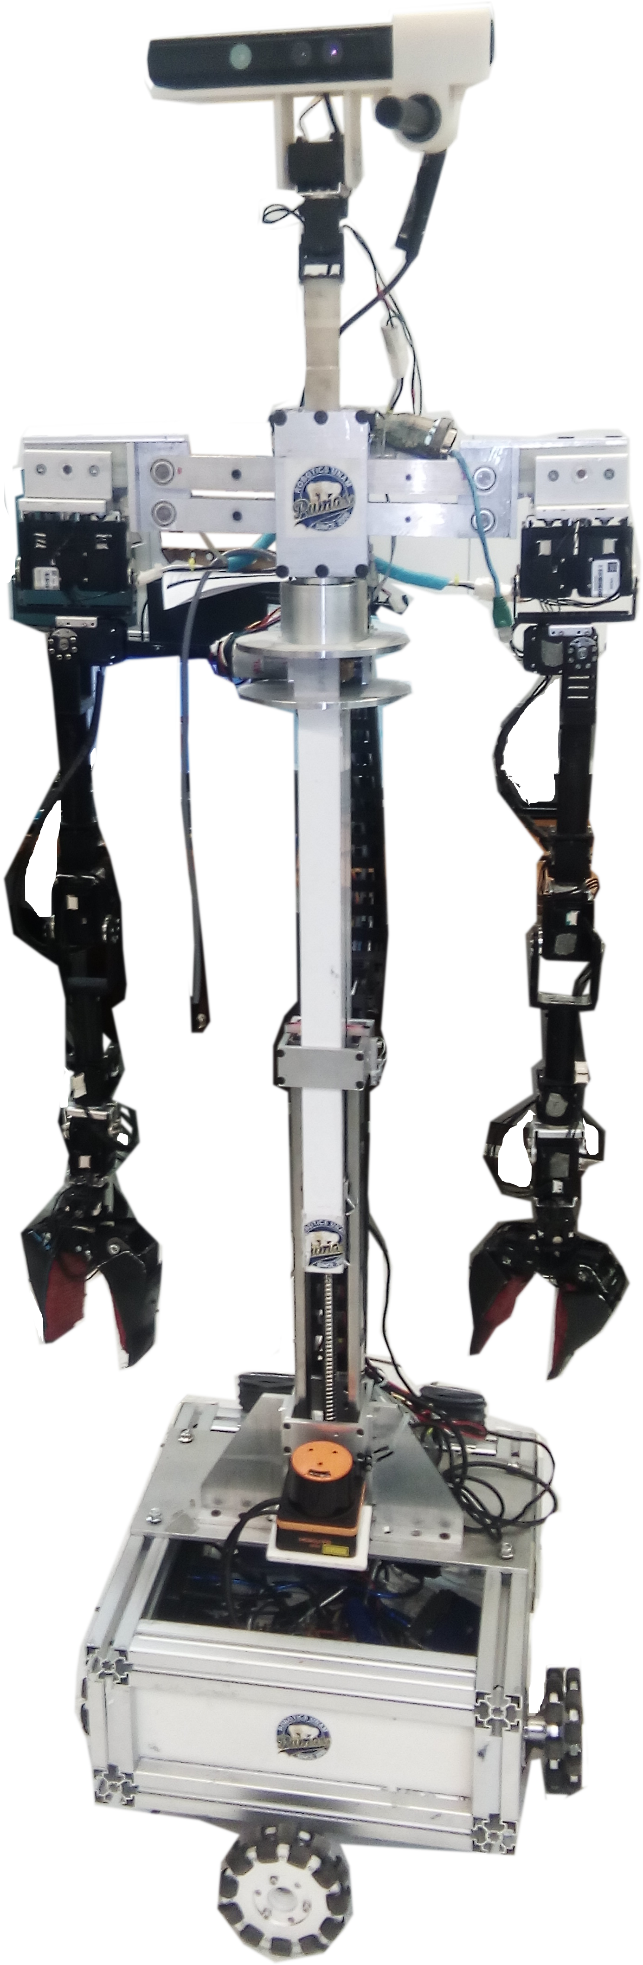
\includegraphics[width=0.3\textwidth]{Figures/Introduction/Justina.png}
\caption{El Robot Justina}
\label{fig:introduction:Justina}
\end{figure}

%Capitulo del Hardware
\chapter{Hardware}
En la siguiente sección mostramos el hardware utilizado para el desarrollo del robót Justina así como especificaciones del mismo y algunas configuraciones que deben seguirse para su correcto funcionamiento.
\section{Diagramas del hardware}

En esta sección se mostrara diagramas pictograficos de lo que es el robot Justina ensamblado y en funcionamiento, así como se indicaran las partes del hardware que utiliza el robot para su funcionamiento.
\subsection{Cuerpo}
%Figura de cuerpo completo de Justina

\begin{center}
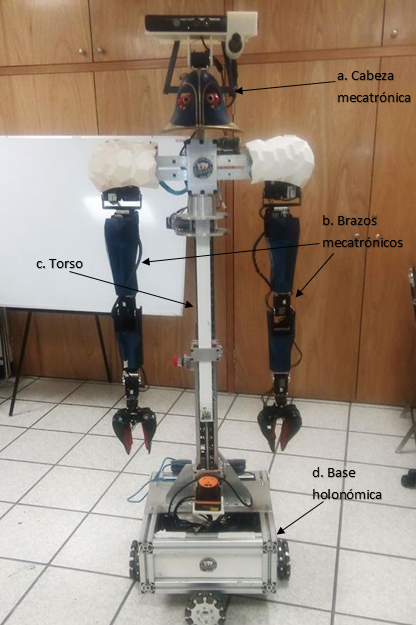
\includegraphics[width=0.6\textwidth]{Figures/Hardware/Diagramas/Cuerpo.png}
\captionof{figure}{El Robot Justina}
\label{fig:Hardware:Diagramas:Justina:Completa}
\end{center}

\subsection{Cabeza}
%Figura de la cabeza de Justina
\begin{center}
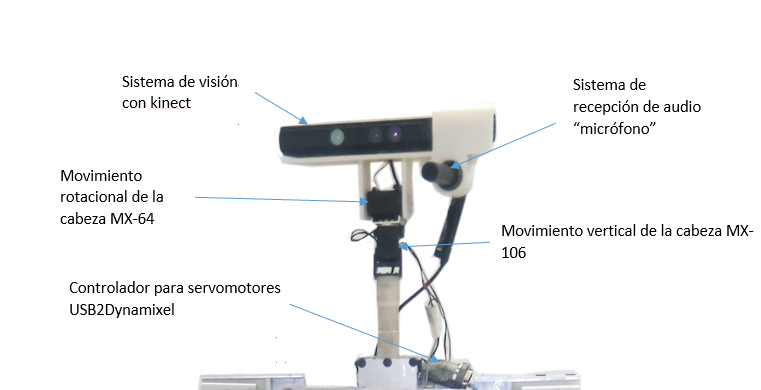
\includegraphics[width=0.8\textwidth]{Figures/Hardware/Diagramas/Cabeza.png}
\captionof{figure}{Cabeza del Robot Justina}
\label{fig:Hardware:Diagramas:Imagen:Cabeza}
\end{center}

\subsection{Brazo}
%Figura del brazo de Justina
\begin{center}
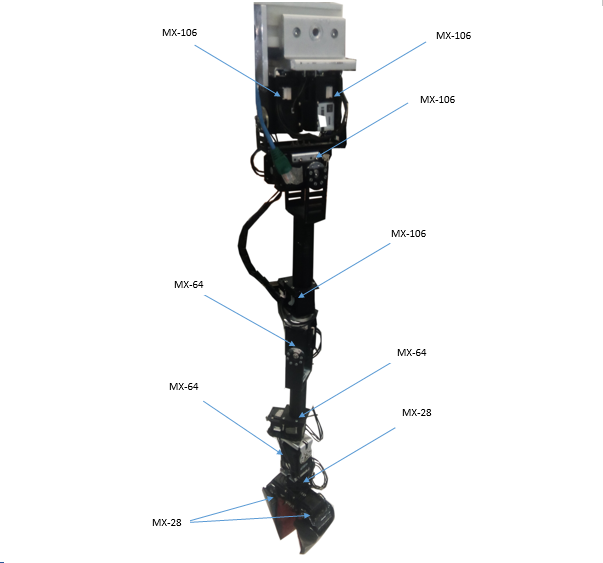
\includegraphics[width=0.8\textwidth]{Figures/Hardware/Diagramas/Brazo.png}
\captionof{figure}{Brazo del Robot Justina}
\label{fig:Hardware:Diagramas:Imagen:Brazo}
\end{center}

 \pagebreak

\section{Partes del hardware}
En ésta sección se mostrar los componentes utilizados para ensamblar al robot Justina y especificadiones tecnnicas como algunas configuraciones y recomendaciones del mismo para su correcto funcionamiento.

\pagebreak

\subsection{Servomotor MX-106}

%Figura
\begin{center}
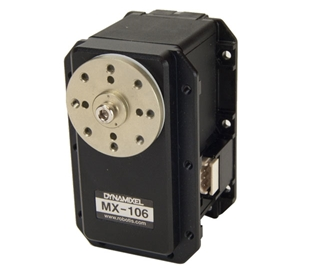
\includegraphics[width=0.45\textwidth]{Figures/Hardware/Partes/MX-106.png}
\captionof{figure}{MX-106}
\label{fig:Hardware:Partes:MX-106}
\end{center}

%Principio de la tabla del MX-106
\begin{table}[H]
\begin{center}
\begin{tabular}{|l|l|l|l|}%Define el número de columnas

\hline
\multicolumn{4}{|c|}{MX-106} \\ \hline %Une un renglon completo 
Voltaje de operación & 14.8[V] & 12[V] & 11.1[V]\\
\hline
\multirow{3}{1cm}{Torque} & 102[kg*cm] & 85.6[Kg*cm] & 81.5[kg*cm]\\ \cline {2-4} %Se hace un renglon multiple
& 10.0[N*m] & 8.4[N*m] & 8[N*m] \\ \cline{1-4}
Velocidad sin carga & 55[RPM] & 45[RPM] & 41[RPM]\\ 
\hline
Masa & \multicolumn{3}{|c|}{153[g]} \\ 
\hline
Medidas & \multicolumn{3}{|c|}{40.2[mm]x65.1[mm]x46[mm]} \\ 
\hline
Resolución & \multicolumn{3}{|c|}{0.088[grados]} \\ 
\hline
Radio de redicción & \multicolumn{3}{|c|}{1/225} \\ 
\hline
Ángulo de operación & \multicolumn{3}{|c|}{360 grados o giro continuo} \\ 
\hline
Corriente máxima & \multicolumn{3}{|c|}{5.2[A] @ 12[V]} \\ 
\hline
Corriente en espera & \multicolumn{3}{|c|}{55[mA]} \\ 
\hline
Temperatura de operación & \multicolumn{3}{|c|}{-5[C]~85[C]} \\ 
\hline
Protocolo & \multicolumn{3}{|c|}{TTL Asynchronous serial} \\ 
\hline
Límite de modulos & \multicolumn{3}{|c|}{254 direcciones validas} \\ 
\hline
Velocidad & \multicolumn{3}{|c|}{8000bps~3Mbps} \\
\hline
Realimentación de posición & \multicolumn{3}{|c|}{Sí} \\
\hline
Realimentación de temperatura & \multicolumn{3}{|c|}{Sí} \\
\hline
Realimentación de voltaje de carga & \multicolumn{3}{|c|}{Sí} \\
\hline
Realimentación de voltaje de entrada & \multicolumn{3}{|c|}{Sí} \\
\hline
PID & \multicolumn{3}{|c|}{Sí} \\
\hline
Materiales & \multicolumn{3}{|c|}{Engranes de metal y cuerpo plastico} \\
\hline
\multirow{4}{1cm}{Lista de controladores} & \multicolumn{3}{|c|}{USB2Dynamixel} \\ \cline {2-4} & \multicolumn{3}{|c|}{CM-530}\\ \cline {2-4} & \multicolumn{3}{|c|}{CM-700}\\ \cline {2-4} & \multicolumn{3}{|c|}{Arbotix}\\ \cline {1-4}
\hline

\end{tabular}
\caption{MX-106}
\label{Datos del MX-106}
\end{center}
\end{table}
%Fin de la tabla
 
 \subsection{Servomotor MX-64}

 %Figura
\begin{center}
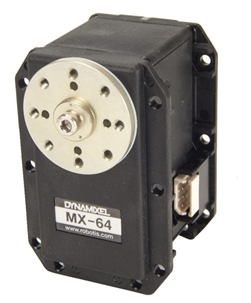
\includegraphics[width=0.3\textwidth]{Figures/Hardware/Partes/MX-64.png}
\captionof{figure}{MX-64}
\label{fig:Hardware:Partes:MX-64}
\end{center}

%Principio de la tabla del MX-64
\begin{table}[H]
\begin{center}
\begin{tabular}{|l|l|l|l|}%Define el número de columnas

\hline
\multicolumn{4}{|c|}{MX-64} \\ \hline %Une un renglon completo 
Voltaje de operación & 14.8[V] & 12[V] & 11.1[V]\\
\hline
\multirow{3}{1cm}{Torque} & 74[kg*cm] & 61[Kg*cm] & 56[kg*cm]\\ \cline {2-4} %Se hace un renglon multiple
& 7.3[N*m] & 6[N*m] & 5.5[N*m] \\ \cline{1-4}
Velocidad sin carga & 78[RPM] & 63[RPM] & 58[RPM]\\ 
\hline
Masa & \multicolumn{3}{|c|}{126[g]} \\ 
\hline
Medidas & \multicolumn{3}{|c|}{40.2[mm]x61.1[mm]x41[mm]} \\ 
\hline
Resolución & \multicolumn{3}{|c|}{0.088[grados]} \\ 
\hline
Radio de redicción & \multicolumn{3}{|c|}{1/200} \\ 
\hline
Ángulo de operación & \multicolumn{3}{|c|}{360 grados o giro continuo} \\ 
\hline
Corriente máxima & \multicolumn{3}{|c|}{4.1[A] @ 12[V]} \\ 
\hline
Corriente en espera & \multicolumn{3}{|c|}{100[mA]} \\ 
\hline
Temperatura de operación & \multicolumn{3}{|c|}{-5[C]~85[C]} \\ 
\hline
Protocolo & \multicolumn{3}{|c|}{TTL Asynchronous serial} \\ 
\hline
Límite de modulos & \multicolumn{3}{|c|}{254 direcciones validas} \\ 
\hline
Velocidad de transmisión & \multicolumn{3}{|c|}{8000bps~3Mbps} \\
\hline
Realimentación de posición & \multicolumn{3}{|c|}{Sí} \\
\hline
Realimentación de temperatura & \multicolumn{3}{|c|}{Sí} \\
\hline
Realimentación de voltaje de carga & \multicolumn{3}{|c|}{Sí} \\
\hline
Realimentación de voltaje de entrada & \multicolumn{3}{|c|}{Sí} \\
\hline
PID & \multicolumn{3}{|c|}{Sí} \\
\hline
Materiales & \multicolumn{3}{|c|}{Engranes de metal y cuerpo plastico} \\
\hline
\multirow{4}{1cm}{Lista de controladores} & \multicolumn{3}{|c|}{USB2Dynamixel} \\ \cline {2-4} & \multicolumn{3}{|c|}{CM-530}\\ \cline {2-4} & \multicolumn{3}{|c|}{CM-700}\\ \cline {2-4} & \multicolumn{3}{|c|}{Arbotix}\\ \cline {1-4}
\hline

\end{tabular}
\caption{MX-64}
\label{Datos del MX-64}
\end{center}
\end{table}
%Fin de la tabla

\subsection{Servomotor MX-28}

%Figura
\begin{center}
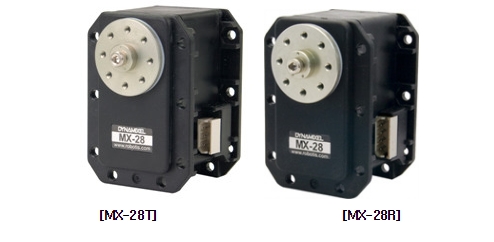
\includegraphics[width=0.7\textwidth]{Figures/Hardware/Partes/MX-28.png}
\captionof{figure}{MX-28}
\label{fig:Hardware:Partes:MX-28}
\end{center}

%Principio de la tabla
\begin{table}[H]
\begin{center}
\begin{tabular}{|l|l|l|l|}%Define el número de columnas

\hline
\multicolumn{4}{|c|}{MX-28} \\ \hline %Une un renglon completo 
Voltaje de operación & 14.8[V] & 12[V] & 11.1[V]\\
\hline
\multirow{3}{1cm}{Torque} & 31[kg*cm] & 25.5[Kg*cm] & 23.4[kg*cm]\\ \cline {2-4} %Se hace un renglon multiple
& 3.1[N*m] & 2.5[N*m] & 2.3[N*m] \\ \cline{1-4}
Velocidad sin carga & 67[RPM] & 55[RPM] & 50[RPM]\\ 
\hline
Masa & \multicolumn{3}{|c|}{72[g]} \\ 
\hline
Medidas & \multicolumn{3}{|c|}{35.6[mm]x50.6[mm]x35.5[mm]} \\ 
\hline
Resolución & \multicolumn{3}{|c|}{0.088[grados]} \\ 
\hline
Radio de redicción & \multicolumn{3}{|c|}{193:1} \\ 
\hline
Ángulo de operación & \multicolumn{3}{|c|}{360 grados o giro continuo} \\ 
\hline
Corriente máxima & \multicolumn{3}{|c|}{1.4[A] @ 12[V]} \\ 
\hline
Corriente en espera & \multicolumn{3}{|c|}{100[mA]} \\ 
\hline
Temperatura de operación & \multicolumn{3}{|c|}{-5[C]~80[C]} \\ 
\hline
Protocolo & \multicolumn{3}{|c|}{TTL Asynchronous serial} \\ 
\hline
Límite de modulos & \multicolumn{3}{|c|}{254 direcciones validas} \\ 
\hline
Velocidad de transmisión & \multicolumn{3}{|c|}{8000bps~3Mbps} \\
\hline
Realimentación de posición & \multicolumn{3}{|c|}{Sí} \\
\hline
Realimentación de temperatura & \multicolumn{3}{|c|}{Sí} \\
\hline
Realimentación de voltaje de carga & \multicolumn{3}{|c|}{Sí} \\
\hline
Realimentación de voltaje de entrada & \multicolumn{3}{|c|}{Sí} \\
\hline
PID & \multicolumn{3}{|c|}{Sí} \\
\hline
Materiales & \multicolumn{3}{|c|}{Engranes de metal y cuerpo plastico} \\
\hline
\multirow{4}{1cm}{Lista de controladores} & \multicolumn{3}{|c|}{USB2Dynamixel} \\ \cline {2-4} & \multicolumn{3}{|c|}{CM-530}\\ \cline {2-4} & \multicolumn{3}{|c|}{CM-700}\\ \cline {2-4} & \multicolumn{3}{|c|}{Open CM 9}\\ \cline {1-4}
\hline

\end{tabular}
\caption{MX-28}
\label{Datos del MX-28}
\end{center}
\end{table}
%Fin de la tabla

\subsection{USB2Dynamixel adapter}

%Figura del Dynamixel
\begin{center}
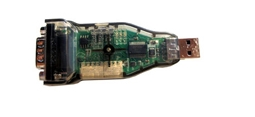
\includegraphics[width=0.8\textwidth]{Figures/Hardware/Partes/Dynamixel.png}
\captionof{figure}{Adaptador USBDynamixel}
\label{fig:Hardware:Partes:Dynamixel}
\end{center}

¡Controlar una red de Robotics Dynamixels desde el puerto USB de la computador!\\
El adaptador USB2Dynamixel tiene tres opciones de salida:\\
\\
-Nivel TTL RS232: conector de 3 pines, usado con un Dynamixel serie AX y MX-T\\

AX-12A\\
AX-18A\\
AX-12W\\
MX-28T\\
MX-64T\\
MX-106T\\
\\

-S485: conector de 4 pines, usado con RX, EX y MX-R de la serie Dynamixel\\

RX-24F\\
RX-28\\
RX-64\\
RX-28R\\
MX-64R\\
MX-106R\\
EX-106\\


\subsection{Roboclaw 2x30A}

%Figura
\begin{center}
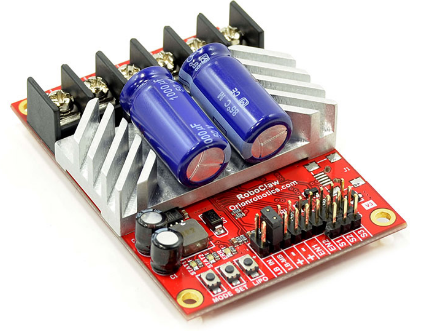
\includegraphics[width=0.6\textwidth]{Figures/Hardware/Partes/Roboclaw_2x30A.png}
\captionof{figure}{Roboclaw 2x30A}
\label{fig:Hardware:Partes:Roboclaw:2x30A}
\end{center}


%Principio de la tabla
\begin{table}[H]
\begin{center}
\begin{tabular}{|l|l|}%Define el número de columnas


\hline
\multicolumn{2}{|c|}{Roboclaw 2x30A} \\ \hline %Une un renglon completo 
Canales para motor & \multicolumn{1}{|c|}{2}\\ \hline
Voltaje de operacion & \multicolumn{1}{|c|}{6[V] a 34[V]}\\ \hline
corriente continua de salida & \multicolumn{1}{|c|}{20[A]}\\ \hline
pico de corriente de salida & \multicolumn{1}{|c|}{60[A]}\\ \hline
5V BEC(1) corriente máxima & \multicolumn{1}{|c|}{3[A]}\\ \hline
Ancho & \multicolumn{1}{|c|}{5.2[cm]}\\ \hline
Largo & \multicolumn{1}{|c|}{7.4[cm]}\\ \hline
Peso & \multicolumn{1}{|c|}{63[g]}\\ \hline

\end{tabular}
\caption{Roboclaw 2x30A}
\label{Datos del Roboclaw}
\end{center}
\end{table}
%Fin de la tabla

\subsection{Roboclaw 2x15A}

%Figura
\begin{center}
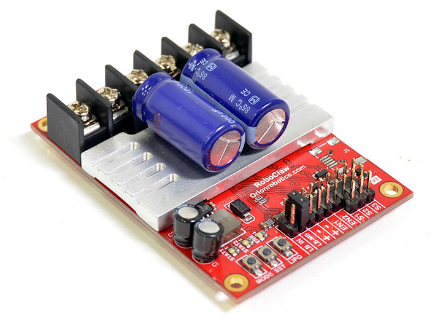
\includegraphics[width=0.7\textwidth]{Figures/Hardware/Partes/Roboclaw_2x15A.png}
\captionof{figure}{Roboclaw 2x15A}
\label{fig:Hardware:Partes:Roboclaw:2x15A}
\end{center}

%Principio de la tabla
\begin{table}[H]
\begin{center}
\begin{tabular}{|l|l|}%Define el número de columnas


\hline
\multicolumn{2}{|c|}{Roboclaw 2x15A} \\ \hline %Une un renglon completo 
Canales para motor & \multicolumn{1}{|c|}{2}\\ \hline
Voltaje de operacion & \multicolumn{1}{|c|}{6[V] a 34[V]}\\ \hline
corriente continua de salida & \multicolumn{1}{|c|}{15[A]}\\ \hline
pico de corriente de salida & \multicolumn{1}{|c|}{30[A]}\\ \hline
5V BEC(1) corriente máxima & \multicolumn{1}{|c|}{3[A]}\\ \hline
Ancho & \multicolumn{1}{|c|}{5.2[cm]}\\ \hline
Largo & \multicolumn{1}{|c|}{7.4[cm]}\\ \hline
Peso & \multicolumn{1}{|c|}{54[g]}\\ \hline

\end{tabular}
\caption{Roboclaw 2x15A}
\label{Datos del Roboclaw}
\end{center}
\end{table}
%Fin de la tabla

%Empiesan los consejos y conexiones 
La siguiente información comprende para las dos RoboClaws antes mencionadas \\
\\
Precauciones\\
Estas son precauciones sumamente importantes que se deberán seguir para evitar daños a la Roboclaw y los sistemas conectados.\\
\\
1. Desconectar la terminal negativa de la alimentación no es la mejor forma para apagar el motor. Si conectas cualquier entrada o salida a la Roboclaw obtienes un ciclo de tierra a los pines de entrada/salida como resultado. Puede causar daños a la Roboclaw y cualquier dispositivo conectado. Para apagar el controlador del motor debe removerse primero la conexión positiva de la alimentación después de que los motores dejen de moverse.\\
\\
2. El motor de DC puede trabajar como un generador cuando este gira. Un robot empieza a ser empujado o apagado con un momento hacia adelante, puede crearse suficiente voltaje lógico de la Roboclaw que pueden entrar en un estado inseguro. Siempre detenga el motor antes de apagar la Roboclaw.\\
\\
3. Apagar en caso de emergencia, un interruptor y/o contacto de un tamaño adecuado debe ser utilizado. debido a que la potencia puede ser desconectada en cualquier momento este no debería ser una ruta para la regeneración.Se debe usar un diodo de clase correcta para hacer un puente entre el apagador y el contacto.\\
\\
4. Dependiendo del modelo de RoboClaw hay un requisito mínimo de potencia de al menos 6V. Bajo cargas pesadas, si la batería lógica y la batería principal se combinan, pueden suceder caídas de tensión. Esto puede causar un comportamiento errático de la RoboClaw.\\
Vista general de los conectores\\
\\
En el control principal de entrada/salida, están puestos para una fácil conectividad para controlar dispositivos como controladores RC. Los cabezales están también arreglados para proveer un fácil acceso a tierra  y alimentación para suministrar poder a controladores externos.

\begin{center}
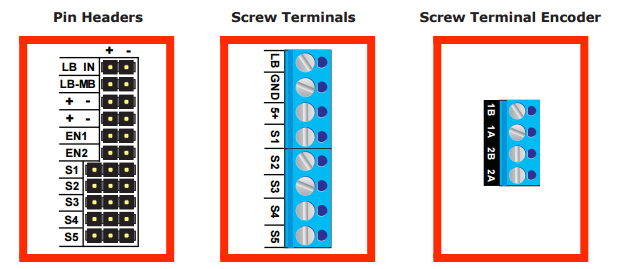
\includegraphics[width=0.9\textwidth]{Figures/Hardware/Partes/Pines.png}
\captionof{figure}{Configuración de pines}
\label{fig:Hardware:Partes:Pines}
\end{center}


Bateria lógica (LB IN)\\
La parte lógica de la RoboClaw puede ser alimentada por una batería secundaria conectada a LB IN. La terminal positiva (+) está localizada al borde de la tarjeta y la tierra (-) es el pin más cercano al disipador. Remueva el jumper LB-MB para que la batería secundaría pueda ser usada.\\
\\
Encoder power (+ -)\\
Los pines marcados como (+) y (–) son los pines de alimentación  de los encoders. El positivo (+) está localizado al borde de la tarjeta y la fuente +5VDC. El pin de tierra (-) está cercano al disipador. En todos los modelos ST la alimentación debe venir del único borne de 5v  y a GND\\
\\
Entradas de los encoder (EN1 / EN2 – 1B / 1A / 2B / 2A)\\ 
EN1 y EN2 son las entradas de los enconders en versión pin del RoboClaw. 1B, 1A, 2B y 2A son las entradas de los encoders a los bornes de la RoboClaw. El canal A de ambos EN1 y EN2 están localizados en los pines del borde de la tarjeta. Los pines del canal B están localizados cercanos al disipador en los pines. Los canales A y B están debidamente etiquetados en los bornes.\\
\\
Cuando conectes los encoders asegúrese que el canal para la dirección de giro esté conectado en A. si un encoder es llevado hacia atras a el otro, tendras un contador interno que contara hacía adelante y hacia atrás. \\
\\
Control de entradas (S1 / S2 / S3 / S4 / S5)\\
S1, S2, S3, S4 y S5 están configuradas para pines de servo estandar de estilo (tipo) entrada/salida (excepto en modelos ST), +5V y GND. S1 y S2 son las entradas  de los modos de control serial, analógico y RC. S3, S4 y S5 pueden ser usadas como entrada de corte de emergencia o como salidas de control de voltaje.\\
\\
Bornes de la batería principal\\
La alimentación de entrada principal puede ser desde 6VDC a 34VDC en la RoboClaw estándar y de 10.5VDC a 60VDC en la Roboclaw de alto voltaje. Las conexiones son hechas en los bornes principales (+) y (-). El símbolo de mas (+) marca la terminal positiva y el negativo (–) marca la terminal negativa. El cableado de la batería principal debe ser lo más corto posible \\
\\
Desconectar\\
La batería principal debe ser desconectada en caso de situaciones donde se salga de control y la energía necesite ser cortada. El interruptor debe estar estimado para manejar la máxima corriente y voltaje de la batería. Esto puede variar dependiendo del tipo de motores y/o la fuente de alimentación que se este utilizando.\\
\\
Bornes del motor\\
Los bornes del motor están hechos con M1A/M1B para el canal 1 y M2A/M2B para el canal 2. Para que ambos motores giren en la misma dirección, el cableado de uno de los motores debe ser contrario hacia el otro en un robot diferencial típico. El cableado de los motores y la batería deben ser lo más cortos posibles. Los cables largos pueden incrementar la inductancia y por lo tanto incrementan potencialmente los picos de voltaje perjudiciales.\\
\\
Leds de estado y error\\
La Roboclaw tiene tres leds. Dos leds de estado, STAT1 y STAT2, y un led de error ERR. Cuando la Roboclaw es alimentada por primera vez, hasta los 3 leds deben parpadear brevemente para indicar que todos los led están funcionando. Los leds se comportaran diferentemente dependiendo en qué modo la Roboclaw está ajustada.\\
\\
\\
Cableado básico\\
El diagrama de cableado de abajo ilustra la batería básica y conexiones de motor para la Roboclaw. M1A y M1B es el canal de motor 1, junto a M2A y M2B como canal de motor 2.\\

%Figura
\begin{center}
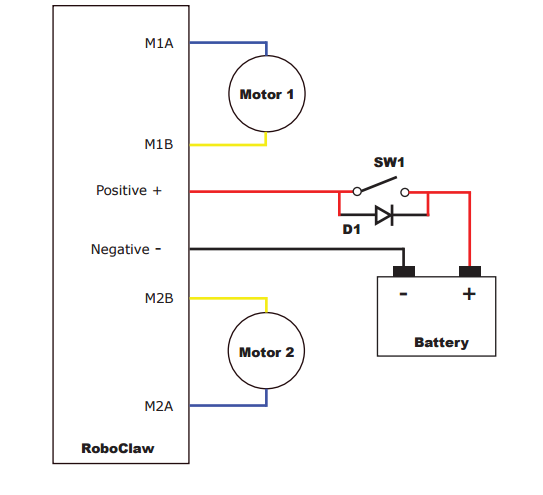
\includegraphics[width=0.8\textwidth]{Figures/Hardware/Partes/Motores.png}
\captionof{figure}{Conexion basica de motores}
\label{fig:Hardware:Partes:Motores}
\end{center}

Nunca desconecte la terminal negativa de la batería antes de desconectar la positiva.\\
\\
Modos de la Roboclaw\\ 
Hay 4 modos principal totalmente variables con 14 modos en total. Cada modo habilita la Roboclaw para ser controlada en una forma específica. La lista a continuación explica cada modo y su aplicación.\\
El USB puede ser conectado en cualquier modo. Cuando la Roboclaw no está en modo USB serie, comandos del pack serial  pueden ser usados para leer información de estados y configuraciones de ajuste, sin embargo los comandos de movimiento de los motores no funcionaran. Cuando en el modo pack serial si otro dispositivo como un arduino es conectado en los pines S1 y S2, y se envían comandos a la Roboclaw, ambos comandos son ejecuatados.\\
\\
1. Modo RC 1 y 2- Con el modo RC la Roboclaw puede ser controlada por cualquier sistema de radio RC. El modo de entrada RC también permite microcontroladores de baja potencia como sello básico de control a la Roboclaw. La Roboclaw espera pulsos de entrada al servo para controlar la dirección y velocidad. Muy similar como regular un servo.\\
\\
2. Modo análogo 3 y 4 – El modo Análogo usa una señal analógica de 0v a 2v para controlar la velocidad y dirección de cada motor. La Roboclaw puede ser controlada usando un potenciómetro o un PWM filtrado por un microcontrolador. El modo análogo es ideal para interfaces de la Roboclaw con sistemas de posicionamiento con joysticks u otro hardware de interface sin microcontrolador. El modo análogo puede usar encoders si tiene la configuración indicada.\\
\\
3. Modo serial estándar 5 y 6 – En el modo serial estándar la Roboclaw espera datos nivel TTL serial del RS-232 para controlar dirección y velocidad de cada motor. El serial estándar es típicamente usado para controlar la Roboclaw desde un microcontrolador o PC. Si se usa una PC, un MAX232 o un circuito convertidor de nivel equivalente debe ser usado desde la Roboclaw la cual sólo trabaja con entradas de nivel TTL. El serial estándar incluye un modo de selección esclavo el cual permite controlar múltiples Roboclaw por una señal desde el puerto RS-232 (PC o microcontrolador). El serial estándar es un formato de un solo camino, la Roboclaw sólo recibe datos. Los encoders no tienen soporte  con el modo serial estándar.\\
\\
4. Modo serial por paquetes del 7 al 14 – En el modo serial de paquetes la Roboclaw espera datos de nivel TTL serial del RS-323 para controlar dirección y velocidad de cada motor. Los paquetes serial son típicamente usados para controlar la Roboclaw desde un microcontrolador o PC. Si se usa una PC, un MAX232 o un circuito convertidor equivalente debe ser usado desde la Roboclaw ya que trabaja sólo con entradas de nivel TTL. En el modo seria por paquetes cada Roboclaw tiene asignada una dirección única. Existen 8 direcciones disponibles. Esto significa que hasta 8 Roboclaws pueden ser usadas en el mismo puerto serial. Los encoders tienen soporte en éste modo.\\
\\
5. Control USB – El USB puede ser conectado en cualquier modo. Cuando la Roboclaw no está en modo serial por paquetes los comandos serial pueden ser utilizados para leer información de estados y/o configurar ajustes, sin embargo los comandos de movimiento del motor no funcionaran. Cuando en el modo serial por paquetes hay otro dispositivo, como por ejemplo arduino, es conectado a los pines S1 y S2, y envía ambos comandos a la Roboclaw y los comandos serial por paquetes USB son ejecutados.\\
%Aquí terminan los consejos de la roboclaw

\vfill

\subsection{Kinect}

%Figura
\begin{center}
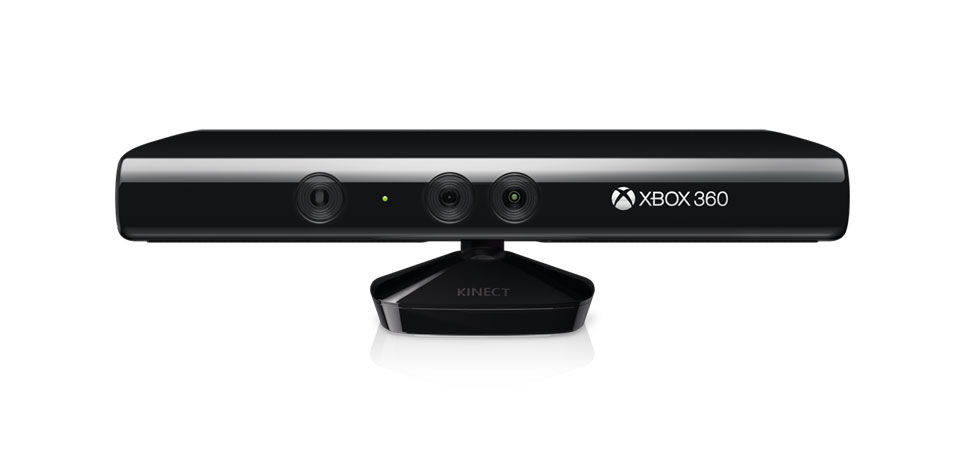
\includegraphics[width=0.9\textwidth]{Figures/Hardware/Partes/Kinect.png}
\captionof{figure}{Kinect}
\label{fig:Hardware:Partes:Kinect}
\end{center}

%Principio de la tabla
\begin{table}[H]
\begin{center}
\begin{tabular}{|l|l|}%Define el número de columnas


\hline
\multicolumn{2}{|c|}{Kinect} \\ \hline %Une un renglon completo 
Caracteristicas & \multicolumn{1}{|c|}{Sensores}\\ \hline
Campo de visión & \multicolumn{1}{|c|}{57.5grados horizontal por 43.5grados vertical}\\ \hline
Profundidad resoluble& \multicolumn{1}{|c|}{0.8[m]->4.0[m]}\\ \hline
\multirow{3}{1cm}{Flujo de color} & \multicolumn{1}{|c|}{640x480x24 bpp 4:3 RGB} \\  & \multicolumn{1}{|c|}{@ 30fps 640x480x16bpp} \\  & \multicolumn{1}{|c|}{4:3 YUV @ 15fps} \\  \hline
Infrarrojo & \multicolumn{1}{|c|}{Sin flujo IR}\\ \hline
Registro & \multicolumn{1}{|c|}{Color <-> ruta}\\ \hline
Ruta de datos & \multicolumn{1}{|c|}{USB 2.0}\\ \hline
Latencia & \multicolumn{1}{|c|}{~90 ms con procesos}\\ \hline
Motor de inclinación & \multicolumn{1}{|c|}{Sólo vertical}\\ \hline

\end{tabular}
\caption{Kinect}
\label{Datos del Kinect}
\end{center}
\end{table}
%Fin de la tabla

\vfill

\subsection{Cisco-Linksys USB2HUB4 USB 4-Port Hub}

%Figura
\begin{center}
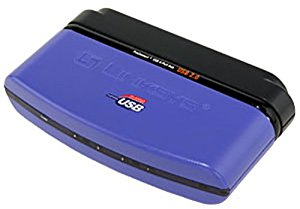
\includegraphics[width=0.5\textwidth]{Figures/Hardware/Partes/Cisco-Linksys.png}
\captionof{figure}{Cisco-Linksys USB2HUB4 USB 4-Port Hub}
\label{fig:Hardware:Partes:Cisco}
\end{center}

%Principio de la tabla
\begin{table}[H]
\begin{center}
\begin{tabular}{|l|l|}%Define el número de columnas


\hline
\multicolumn{2}{|c|}{USB2HUB4} \\ \hline %Une un renglon completo 
\multirow{3}{1cm}{Estándar} & \multicolumn{1}{|c|}{OHCI}\\ & \multicolumn{1}{|c|}{UHIC}\\ & \multicolumn{1}{|c|}{USB 1.1}\\ & \multicolumn{1}{|c|}{USB 2.0}\\ \hline
Puertos & \multicolumn{1}{|c|}{USB type B Root port}\\ &\multicolumn{1}{|c|}{4 USB type A device ports}\\ \hline
Número máximo de dispositivos & \multicolumn{1}{|c|}{127}\\ \hline
Cable & \multicolumn{1}{|c|}{Shielded USB 2.0}\\ \hline
\multicolumn{2}{|c|}{Environmental}\\ \hline
Dimensiones & \multicolumn{1}{|c|}{4.52"x0.75"x2.675"}\\ \hline
Masa & \multicolumn{1}{|c|}{70[g]}\\ \hline
Alimentación & \multicolumn{1}{|c|}{5[V] DC a 2.4[A]}\\ \hline
Temperatura de operación & \multicolumn{1}{|c|}{0 a 70 grados}\\ \hline
Temperatura en almacenamiento & \multicolumn{1}{|c|}{-20 a 176 grados}\\ \hline
Humedad de operación & \multicolumn{1}{|c|}{0 a 95\% sin condensación}\\ \hline
Humedad en almacenamiento & \multicolumn{1}{|c|}{0 a 95\% sin condensación}\\ \hline

\end{tabular}
\caption{USB2HUB4}
\label{Datos del USB2HUB4}
\end{center}
\end{table}
%Fin de la tabla

\subsection{Hokuyo UHG-08LX}

%Figura
\begin{center}
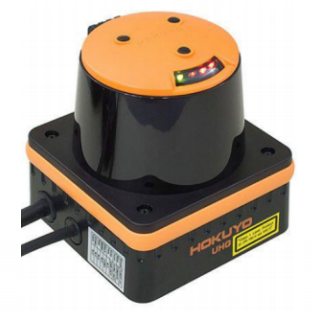
\includegraphics[width=0.5\textwidth]{Figures/Hardware/Partes/Hokuyo.png}
\captionof{figure}{Hokuyo UHG-08LX}
\label{fig:Hardware:Partes:Hokuyo:UHG-08LX}
\end{center}

%Principio de la tabla
\begin{table}[H]
\begin{center}
\begin{tabular}{|l|l|}%Define el número de columnas


\hline
\multicolumn{2}{|c|}{Hokuyo UHG-08LX Scanning Laser} \\ \hline %Une un renglon completo 
Alimentación &  \multicolumn{1}{|c|}{12[V]}\\ \hline
Rango de detección & \multicolumn{1}{|c|}{De 20 a 8000[mm]}\\ \hline
Exactitud & \multicolumn{1}{|c|}{De 100 a 1000[mm]}\\ \hline
Resolución angular & \multicolumn{1}{|c|}{0.36grados(360grados/1,024 pasos)}\\ \hline

Fuente de luz & \multicolumn{1}{|c|}{Diodo laser semiconductor }\\ \hline
Tiempo de escaneo & \multicolumn{1}{|c|}{67[msec/scan]}\\ \hline
Nivel de sonido & \multicolumn{1}{|c|}{menos de 25dB}\\ \hline
Interface & \multicolumn{1}{|c|}{USB2.0 (velocidad completa)}\\ \hline
Salida sincrona & \multicolumn{1}{|c|}{NPN colector abierto}\\ \hline
Comando del sistema & \multicolumn{1}{|c|}{Comanda diseñado exclusivamente SCIP ver. 2.0}\\ \hline
Conexión & \multicolumn{1}{|c|}{Salida de voltaje y sincronia: 2}\\ \hline
Iluminación ambiente & \multicolumn{1}{|c|}{Lampara de alogeno/mercurio: 10,000lx o menos, florecente: 6,000lx(máx)}\\ \hline
Ambiente (temperatura/humedad) & \multicolumn{1}{|c|}{-10 a 50grados C, menos del 85\% RH}\\ \hline
Resistencia a la vibración & \multicolumn{1}{|c|}{Amplitud doble 1.5[mm], de 10 a 55[Hz], 2 veces en cada dirección X, Y y Z}\\ \hline
Resistencia al impacto & \multicolumn{1}{|c|}{196[m/s], 10 veces en las direcciones X, Y y Z}\\ \hline
Peso & \multicolumn{1}{|c|}{Aprox. 500[g](con el cable conectado)}\\ \hline

\end{tabular}
\caption{Hakuyo UHG-08LX}
\label{Datos del Hokuyo}
\end{center}
\end{table}
%Fin de la tabla

\subsection{Microfono RODE}

%Figura
\begin{center}
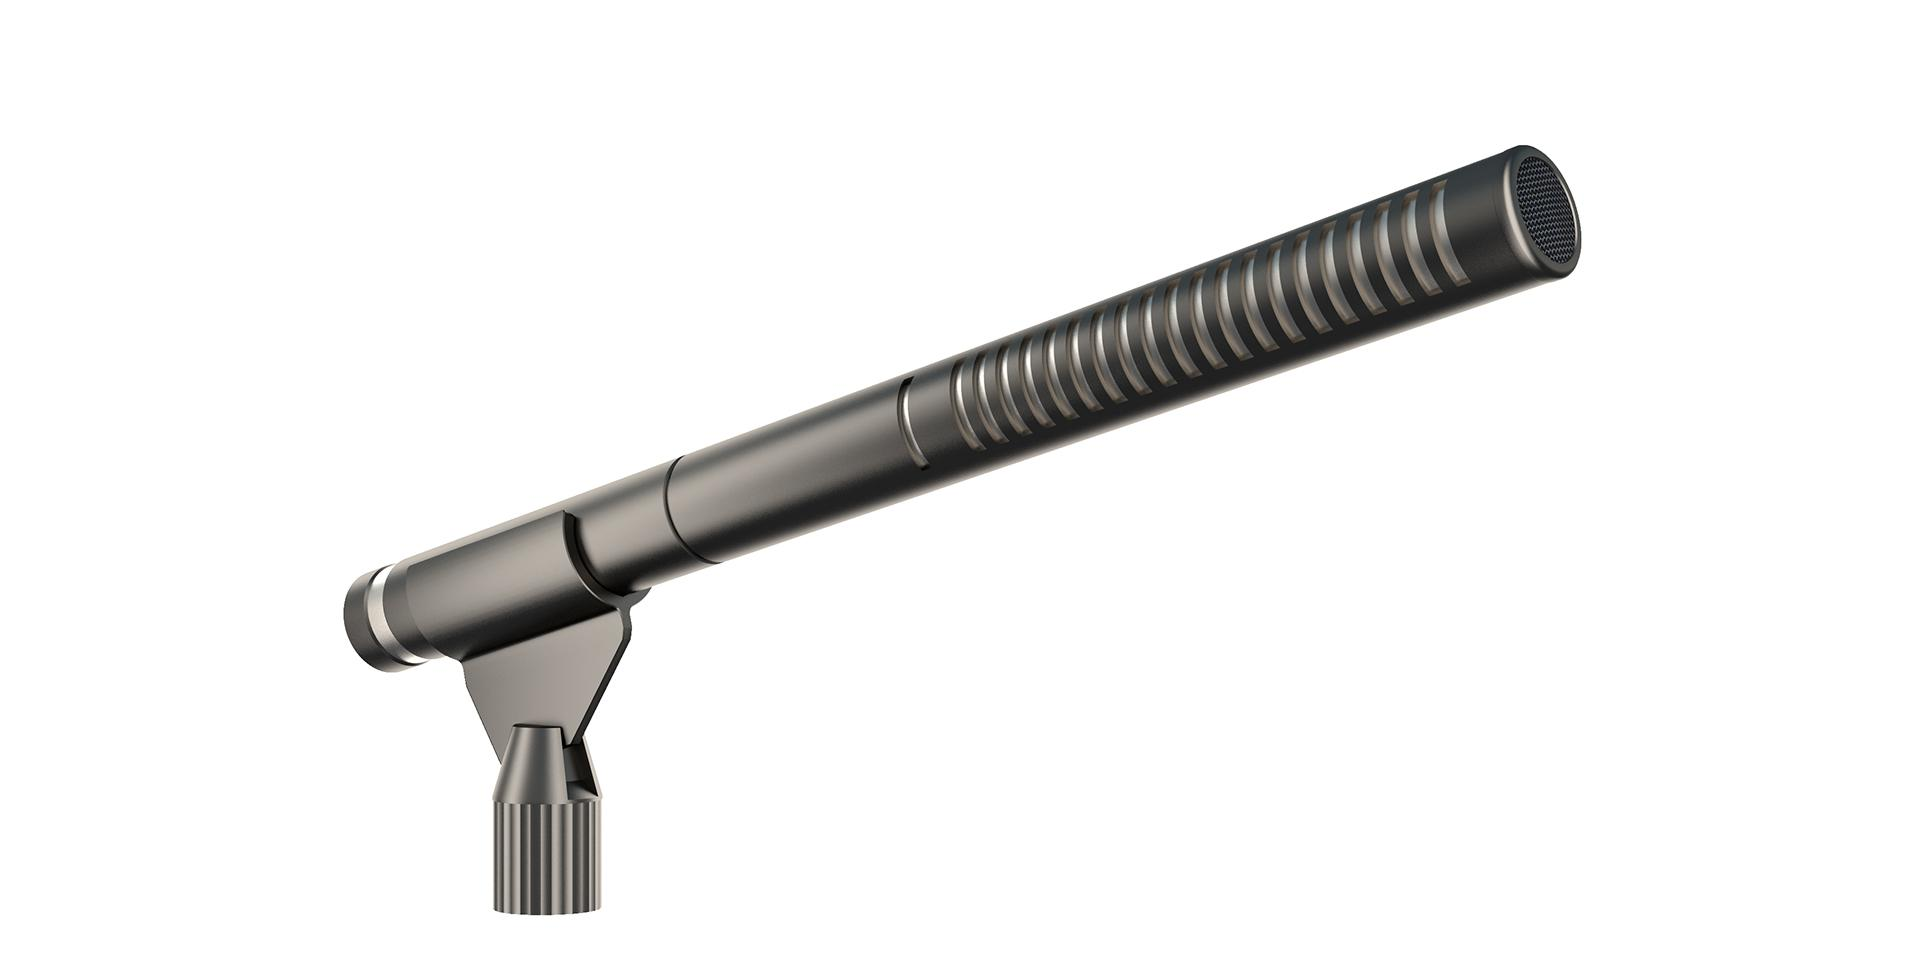
\includegraphics[width=0.7\textwidth]{Figures/Hardware/Partes/Rode.jpg}
\captionof{figure}{Microfono Rode NTG-2}
\label{fig:Hardware:Partes:Microfono:Rode}
\end{center}

%Principio de la tabla
\begin{table}[H]
\begin{center}
\begin{tabular}{|l|l|}%Define el número de columnas

\hline
\multicolumn{2}{|c|}{Microfono Rode NTG-2} \\ \hline %Une un renglon completo 
Principio acustico &  \multicolumn{1}{|c|}{Line Gradient}\\ \hline
Electronica & \multicolumn{1}{|c|}{Conversor de impedancia JFET con un transformador de saldia balanceado}\\ \hline
Capsula & \multicolumn{1}{|c|}{0.50"}\\ \hline
Tipo de dirección & \multicolumn{1}{|c|}{End}\\ \hline
Rango de frecuencia & \multicolumn{1}{|c|}{20Hz-20kHz}\\ \hline
Impedancia de salida & \multicolumn{1}{|c|}{250[ohms]}\\ \hline
Nivel de sonido & \multicolumn{1}{|c|}{131dB SPL(@ 1kHz, 1\% THD en carga de 1kohm)}\\ \hline
Máximo nivel de salida & \multicolumn{1}{|c|}{6.9[mV]}\\ \hline
Sensibilidad & \multicolumn{1}{|c|}{-36.0dB re 1[Volt/pascal] (15[mV] @ 94dB SPL)+/- 2dB}\\ \hline
Nivel de ruido equivalente & \multicolumn{1}{|c|}{18dB-A}\\ \hline
Opciones de alimentación & \multicolumn{1}{|c|}{Pilas AA o P48}\\ \hline
Peso & \multicolumn{1}{|c|}{161[gm]}\\ \hline
Dimensiones & \multicolumn{1}{|c|}{280[mmH]x22[mmW]x22[mmD]}\\ \hline
Salida & \multicolumn{1}{|c|}{XLR}\\ \hline


\end{tabular}
\caption{Microfono Rode}
\label{Microfono Rode}
\end{center}
\end{table}
%Fin de la tabla
\vfill


\subsection{Alimentación bateria Li-po}

Para el robot Justina se utilizan 3 baterias conectadas en paralelo

%Figura
\begin{center}
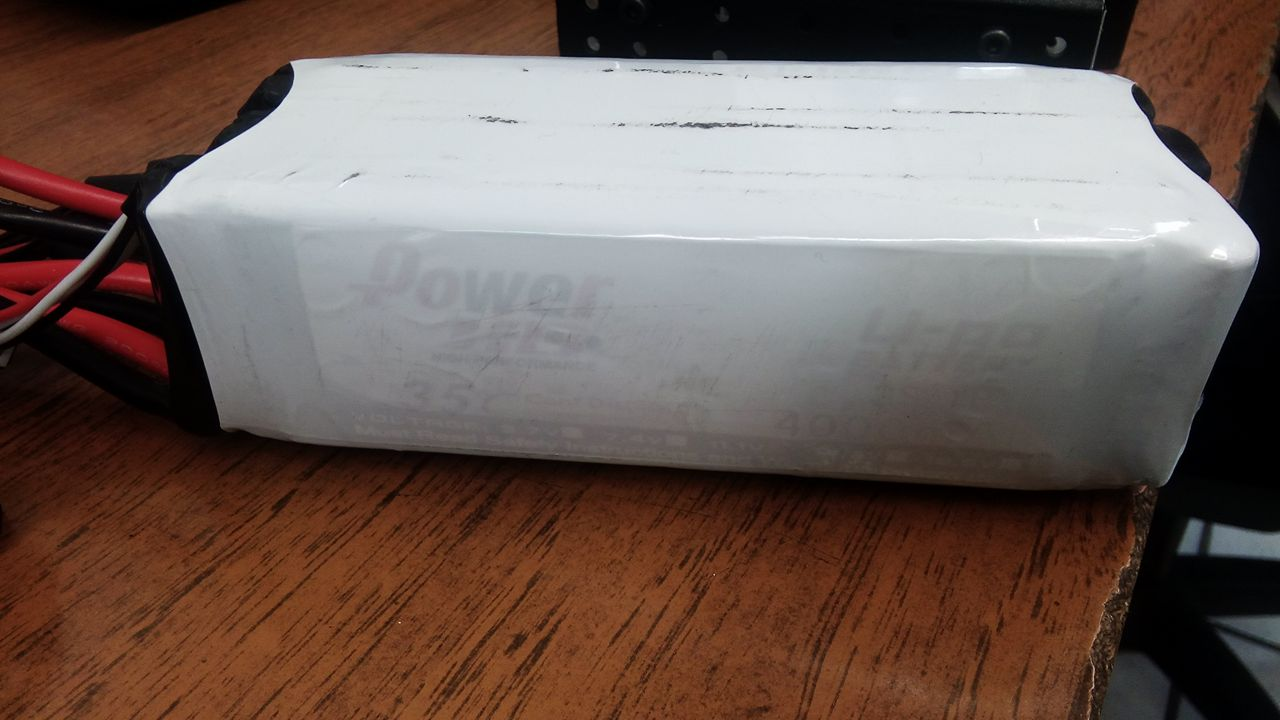
\includegraphics[width=0.7\textwidth]{Figures/Hardware/Partes/Li-po_Battery.jpg}
\captionof{figure}{Bateria Li-po}
\label{fig:Hardware:Partes:Battery}
\end{center}

%Principio de la tabla
\begin{table}[H]
\begin{center}
\begin{tabular}{|l|l|}%Define el número de columnas

\hline
\multicolumn{2}{|c|}{Bateria Li-po 4000mAh a 11.1[V]} \\ \hline %Une un renglon completo 
Voltaje &  \multicolumn{1}{|c|}{11.1[V] en 3 celdas}\\ \hline
Corriente de descarga por hora  & \multicolumn{1}{|c|}{4000[mAh]}\\ \hline
Tasa de descarga & \multicolumn{1}{|c|}{35C}\\ \hline
Plug de carga & \multicolumn{1}{|c|}{JST-XH}\\ \hline
Plug de descarga & \multicolumn{1}{|c|}{"T"}\\ \hline
Medidas & \multicolumn{1}{|c|}{25x46x144[mm]}\\ \hline
Peso & \multicolumn{1}{|c|}{335[gr]}\\ \hline

\end{tabular}
\caption{Bateria Li-po}
\label{Battery}
\end{center}
\end{table}
%Fin de la tabla

%Información sobre la batería LiPo
INSTRUCCIONES DE USO Y SEGURIDAD PARA BATERÍAS LIPO (POLÍMERO DE LITIO)\\
\\
Normas a seguir para evitar cualquier peligro o mal funcionamiento:\\
\\
    Emplee sólo cargadores específicos para baterías de Polímero de Litio (LiPo). En caso contrario puede provocar un incendio que derive en daños personales y/o materiales.\\
    Nunca cargue las baterías LiPo sin estar presente. Siempre debe vigilar el proceso para poder reaccionar ante cualquier problema que se pudiese plantear.\\
    Si en cualquier momento observa que una batería Lipo se hincha o derrama líquido, desconéctela y obsérvela durante 15 minutos en un lugar seguro y alejado de cualquier material combustible.\\
    Tenga mucho cuidado de que NUNCA se toquen los dos terminales de la batería, este cortocircuito podría hacer que la batería se incendiase.\\
    Una batería que haya sufrido un golpe, cortocircuito u otro problema puede llegar a incendiarse incluso 10-15 minutos después de haberse producido este hecho. Lleve rápidamente la batería a un lugar seguro y obsérvela durante 15 minutos.\\
    NUNCA almacene sus baterías en un vehículo ni en cualquier lugar donde se puedan alcanzar temperaturas altas. Las temperaturas extremas pueden causar el incendio de la batería.\\
    Tenga mucho cuidado de NO PERFORAR ningún pack de baterías LiPo, puede provocar un incendio.\\
    \\
Proceso de carga:\\
\\
    Nunca cargue las baterías sin vigilarlas y utilice solo cargadores especiales para las baterias de lipo, asi como tener en cuenta el número de elementos que contiene su bateria.\\
    Cargue las baterías en un área segura y aislada de cualquier material inflamable.\\
    Deje enfriar la batería a la temperatura ambiente antes de comenzar la carga.\\
    Valores nominales de una bateria de lipo cargada.\\
\\
    Lipos 2S (2 elementos): entre 8,32 y 8,44V\\
    Lipos 3S (3 elementos): entre 12,48 y 12,66V\\
    Lipos 4S (4 elementos): entre 16,64 y 16,88V\\
\\
Nunca descargue una batería por debajo de 3V por elemento, puede dañar la batería. Para ello debe tener cuidado de no agotarla más de lo debido empleando dispositivos de corte por bajo voltaje o variadores especialmente diseñados para baterías LiPo.\\
\\
Fin de vida de las baterías LiPo:\\
\\
Cuando la capacidad de la batería haya disminuido un 30\%, deberá desecharla. Para ello descárguela a 3V por elemento, aisle sus terminales, envuélvala en plástico y deposítelas en los contenedores especiales para el desecho responsable de pilas.\\

\subsection{Motor-DCX32L GB KL 12V}
Existen 2 tipos de motores DCX32L, el GPX32 LN 16:1 y el GPX32 G1 35:1 los cuales tienen cambios en sus funciones pero escencialmente conservan el diseño.
%Figura
\begin{center}
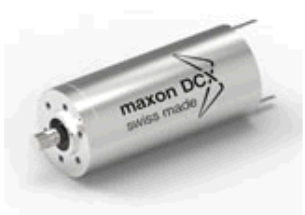
\includegraphics[width=0.5\textwidth]{Figures/Hardware/Partes/DCX32L.png}
\captionof{figure}{Motor DCX32L}
\label{fig:Hardware:Partes:Motor:DCX32L}
\end{center}

%Principio de la tabla GPX32 G1 35:1
%Sensor - ENX16 EASY 1024IMP
\begin{table}[H]
\begin{center}
\begin{tabular}{|l|l|}

\hline
\multicolumn{2}{|c|}{GPX32 G1 35:1}\\ \hline
\multicolumn{2}{|c|}{Funciones}\\ \hline
Gearhead type & \multicolumn{1}{|c|}{Versión estándar}\\ \hline
Redeucción & \multicolumn{1}{|c|}{35:1}\\ \hline
Número de etapas & \multicolumn{1}{|c|}{2}\\ \hline
Conmutación & \multicolumn{1}{|c|}{Graphote brushes}\\ \hline
Fuente de voltaje & \multicolumn{1}{|c|}{Voltaje nominal 12[V]}\\ \hline
Motor bearings & \multicolumn{1}{|c|}{preloaded ball bearing}\\ \hline
Conteos por vuelta & \multicolumn{1}{|c|}{1024}\\ \hline
Hysteresis & \multicolumn{1}{|c|}{0.17m}\\ \hline
\multicolumn{2}{|c|}{Forma y ajuste}\\ \hline
Gear shaft & \multicolumn{1}{|c|}{With flat}\\ \hline
Shaft bore & \multicolumn{1}{|c|}{Without transverse bore}\\ \hline
Shaft length L1 & \multicolumn{1}{|c|}{21[mm]}\\ \hline
Length of flat L2 & \multicolumn{1}{|c|}{12[mm]}\\ \hline
Height of flat D2 & \multicolumn{1}{|c|}{7[mm]}\\ \hline
Gear flange & \multicolumn{1}{|c|}{Standard flange}\\ \hline
Amount of threads & \multicolumn{1}{|c|}{4}\\ \hline
Thread diameter & \multicolumn{1}{|c|}{M3}\\ \hline
Pitch circle diameter TK & \multicolumn{1}{|c|}{26[mm]}\\ \hline
Conexión eléctrica, motor & \multicolumn{1}{|c|}{cable}\\ \hline
Tipo de conector, motor & \multicolumn{1}{|c|}{Sin conector}\\ \hline
Longitud del cable L1 para el motor & \multicolumn{1}{|c|}{200[mm]}\\ \hline
Tipo de cable & \multicolumn{1}{|c|}{AWG18}\\ \hline
Conexión electrica, enconder & \multicolumn{1}{|c|}{Estándar}\\ \hline
Longitud del cable L1 para el encoder & \multicolumn{1}{|c|}{200[mm]}\\ \hline
Tipo de cable para el enconder & \multicolumn{1}{|c|}{TPE ribbon cable}\\ \hline
Tipo de conector, encoder & \multicolumn{1}{|c|}{10-pol 2.54[mm] pin}\\ \hline
Orientación de la conexión (motor) & \multicolumn{1}{|c|}{0 grados}\\ \hline
Orientación de la conexión (enconder) & \multicolumn{1}{|c|}{0 grados}\\ \hline
\multicolumn{2}{|c|}{Your entries}\\ \hline
Voltaje disponible & \multicolumn{1}{|c|}{12[V]}\\ \hline
Velocidad & \multicolumn{1}{|c|}{180[rpm]}\\ \hline
Torque & \multicolumn{1}{|c|}{2000[mNm]}\\ \hline
\multicolumn{2}{|c|}{Valores de el dispositivo con voltaje}\\ \hline
Máx. speed at given load & \multicolumn{1}{|c|}{190[rpm]}\\ \hline
Máximo torque continuo & \multicolumn{1}{|c|}{2440.62[mNm]}\\ \hline
Máxima corriente continua & \multicolumn{1}{|c|}{6[A]}\\ \hline



\end{tabular}
\caption{GPX32 G1 35:1}
\label{GPX32 G1 }
\end{center}
\end{table}
%Fin de la tabla

%Principio de la tabla GPX32 LN 16:1
%Sensor - ENX16 EASY 1024IMP
\begin{table}[H]
\begin{center}
\begin{tabular}{|l|l|}

\hline
\multicolumn{2}{|c|}{GPX32 G1 16:1}\\ \hline
\multicolumn{2}{|c|}{Funciones}\\ \hline
Gearhead type & \multicolumn{1}{|c|}{Nivel de ruido reducido}\\ \hline
Redeucción & \multicolumn{1}{|c|}{16:1}\\ \hline
Número de etapas & \multicolumn{1}{|c|}{2}\\ \hline
Conmutación & \multicolumn{1}{|c|}{Graphote brushes}\\ \hline
Fuente de voltaje & \multicolumn{1}{|c|}{Voltaje nominal 12[V]}\\ \hline
Motor bearings & \multicolumn{1}{|c|}{preloaded ball bearing}\\ \hline
Conteos por vuelta & \multicolumn{1}{|c|}{1024}\\ \hline
Hysteresis & \multicolumn{1}{|c|}{0.17m}\\ \hline
\multicolumn{2}{|c|}{Forma y ajuste}\\ \hline
Gear shaft & \multicolumn{1}{|c|}{With flat}\\ \hline
Shaft bore & \multicolumn{1}{|c|}{Without transverse bore}\\ \hline
Shaft length L1 & \multicolumn{1}{|c|}{21[mm]}\\ \hline
Length of flat L2 & \multicolumn{1}{|c|}{12[mm]}\\ \hline
Height of flat D2 & \multicolumn{1}{|c|}{7[mm]}\\ \hline
Gear flange & \multicolumn{1}{|c|}{Standard flange}\\ \hline
Amount of threads & \multicolumn{1}{|c|}{4}\\ \hline
Thread diameter & \multicolumn{1}{|c|}{M3}\\ \hline
Pitch circle diameter TK & \multicolumn{1}{|c|}{26[mm]}\\ \hline
Conexión eléctrica, motor & \multicolumn{1}{|c|}{Terminal (bent radially)}\\ \hline
Conexión electrica, enconder & \multicolumn{1}{|c|}{Estándar}\\ \hline
Longitud del cable L1 para el encoder & \multicolumn{1}{|c|}{200[mm]}\\ \hline
Tipo de cable para el enconder & \multicolumn{1}{|c|}{TPE ribbon cable}\\ \hline
Tipo de conector, encoder & \multicolumn{1}{|c|}{10-pol 2.54[mm] pin}\\ \hline
Orientación de la conexión (motor) & \multicolumn{1}{|c|}{0 grados}\\ \hline
Orientación de la conexión (enconder) & \multicolumn{1}{|c|}{0 grados}\\ \hline
\multicolumn{2}{|c|}{Your entries}\\ \hline
Voltaje disponible & \multicolumn{1}{|c|}{12[V]}\\ \hline
Velocidad & \multicolumn{1}{|c|}{400[rpm]}\\ \hline
Torque & \multicolumn{1}{|c|}{900[mNm]}\\ \hline
\multicolumn{2}{|c|}{Valores de el dispositivo con voltaje}\\ \hline
Máx. speed at given load & \multicolumn{1}{|c|}{417[rpm]}\\ \hline
Máximo torque continuo & \multicolumn{1}{|c|}{1115.71[mNm]}\\ \hline
Máxima corriente continua & \multicolumn{1}{|c|}{6[A]}\\ \hline

\end{tabular}
\caption{Motor DCX32L}
\label{Motor DCX32L}
\end{center}
\end{table}
%Fin de la tabla

%Principio de la tabla
\begin{table}[H]
\begin{center}
\begin{tabular}{|l|l|}%Define el número de columnas

\hline
\multicolumn{2}{|c|}{Motor - DCX32L GB KL 12V} \\ \hline %Une un renglon completo 
\multicolumn{2}{|c|}{Valores en voltaje nominal} \\ \hline %Une un renglon completo 
Voltaje nominal &  \multicolumn{1}{|c|}{12[V]}\\ \hline
Velocidad sin carga  & \multicolumn{1}{|c|}{7120[rpm]}\\ \hline
Corriente sin carga & \multicolumn{1}{|c|}{274[mA]}\\ \hline
Velocidad nominal & \multicolumn{1}{|c|}{6560[rpm]}\\ \hline
Torque nominal (máx. torque continuo) & \multicolumn{1}{|c|}{89.4[mNm]}\\ \hline
Corriente nominal & \multicolumn{1}{|c|}{6[A]}\\ \hline
Stall Torque & \multicolumn{1}{|c|}{1730[mNm]}\\ \hline
Stall Corriente & \multicolumn{1}{|c|}{111[A]}\\ \hline
Eficiencia máxima & \multicolumn{1}{|c|}{85.5\%}\\ \hline
\multicolumn{2}{|c|}{Caracteristicas} \\ \hline %Une un renglon completo 
Máxima salida de potencia & \multicolumn{1}{|c|}{90.2[W]}\\ \hline
Resistencia de terminal & \multicolumn{1}{|c|}{0.108[Ohm]}\\ \hline
Inductancía de terminal & \multicolumn{1}{|c|}{0.03362[mH]}\\ \hline
Torque constante & \multicolumn{1}{|c|}{15.6[mNm/A]}\\ \hline
Velocidad constante & \multicolumn{1}{|c|}{612[rpm/V]}\\ \hline
Gradiente de velocidad/torque & \multicolumn{1}{|c|}{4.24[rpm/mNm]}\\ \hline
Mechanical time constant & \multicolumn{1}{|c|}{3.44[ms]}\\ \hline
Inercia del rotor & \multicolumn{1}{|c|}{77.6[gcm\^2]}\\ \hline
\multicolumn{2}{|c|}{Datos termicos} \\ \hline %Une un renglon completo 
Resistencia termica housing-ambient & \multicolumn{1}{|c|}{7.28[K/W]}\\ \hline
Resistencia termica winding-housing & \multicolumn{1}{|c|}{2.3[K/W]}\\ \hline
Thermal time constant 0f the winding & \multicolumn{1}{|c|}{45[s]}\\ \hline
Constante de tiempo termica del motor & \multicolumn{1}{|c|}{837[s]}\\ \hline
Temperatura ambiente & \multicolumn{1}{|c|}{-40 a 100[Grados C]}\\ \hline
Max. winding temperatura & \multicolumn{1}{|c|}{155[grados C]}\\ \hline
\multicolumn{2}{|c|}{Datos mecanicos} \\ \hline %Une un renglon completo 
Velocidad máxima permisible & \multicolumn{1}{|c|}{11300[rpm]}\\ \hline
Min. axial play & \multicolumn{1}{|c|}{0[mm]}\\ \hline
Máx. axial play & \multicolumn{1}{|c|}{0.1[mm]}\\ \hline
Radial backlash & \multicolumn{1}{|c|}{0.02[mm]}\\ \hline
Max. axial load (dynamic) & \multicolumn{1}{|c|}{7[N]}\\ \hline
Max. force for press fits & \multicolumn{1}{|c|}{22.6[N]}\\ \hline
Max. radial load & \multicolumn{1}{|c|}{65.3[N]}\\ \hline
\multicolumn{2}{|c|}{Especificaciones} \\ \hline %Une un renglon completo
Número de pares de polos & \multicolumn{1}{|c|}{1}\\ \hline
Número de segmentos del conmutador & \multicolumn{1}{|c|}{11}\\ \hline
Peso & \multicolumn{1}{|c|}{0[mm]}\\ \hline
Nivel de ruido tipico & \multicolumn{1}{|c|}{47dbA}\\ \hline



\end{tabular}
\caption{Motor DCX32L}
\label{Motor DCX32L}
\end{center}
\end{table}
%Fin de la tabla

\subsection{ATX}

%Figura
\begin{center}
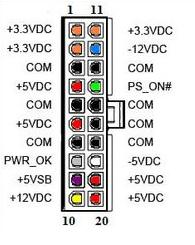
\includegraphics[width=0.3\textwidth]{Figures/Hardware/Partes/ATX.JPG}
\captionof{figure}{Conector ATX}
\label{fig:Hardware:Partes:ATX}
\end{center}


\vfill
\pagebreak

%Empiezan la sección de los diagramas esquematicos del capitulo de hardware
\section{Diagramas esquematicos}
Se muestran los diagramas esquematicos de las conexiones del hardware de Justina.

\pagebreak

\subsection{Diagrama esquematico conexiones generales}

%Figura
\begin{center}
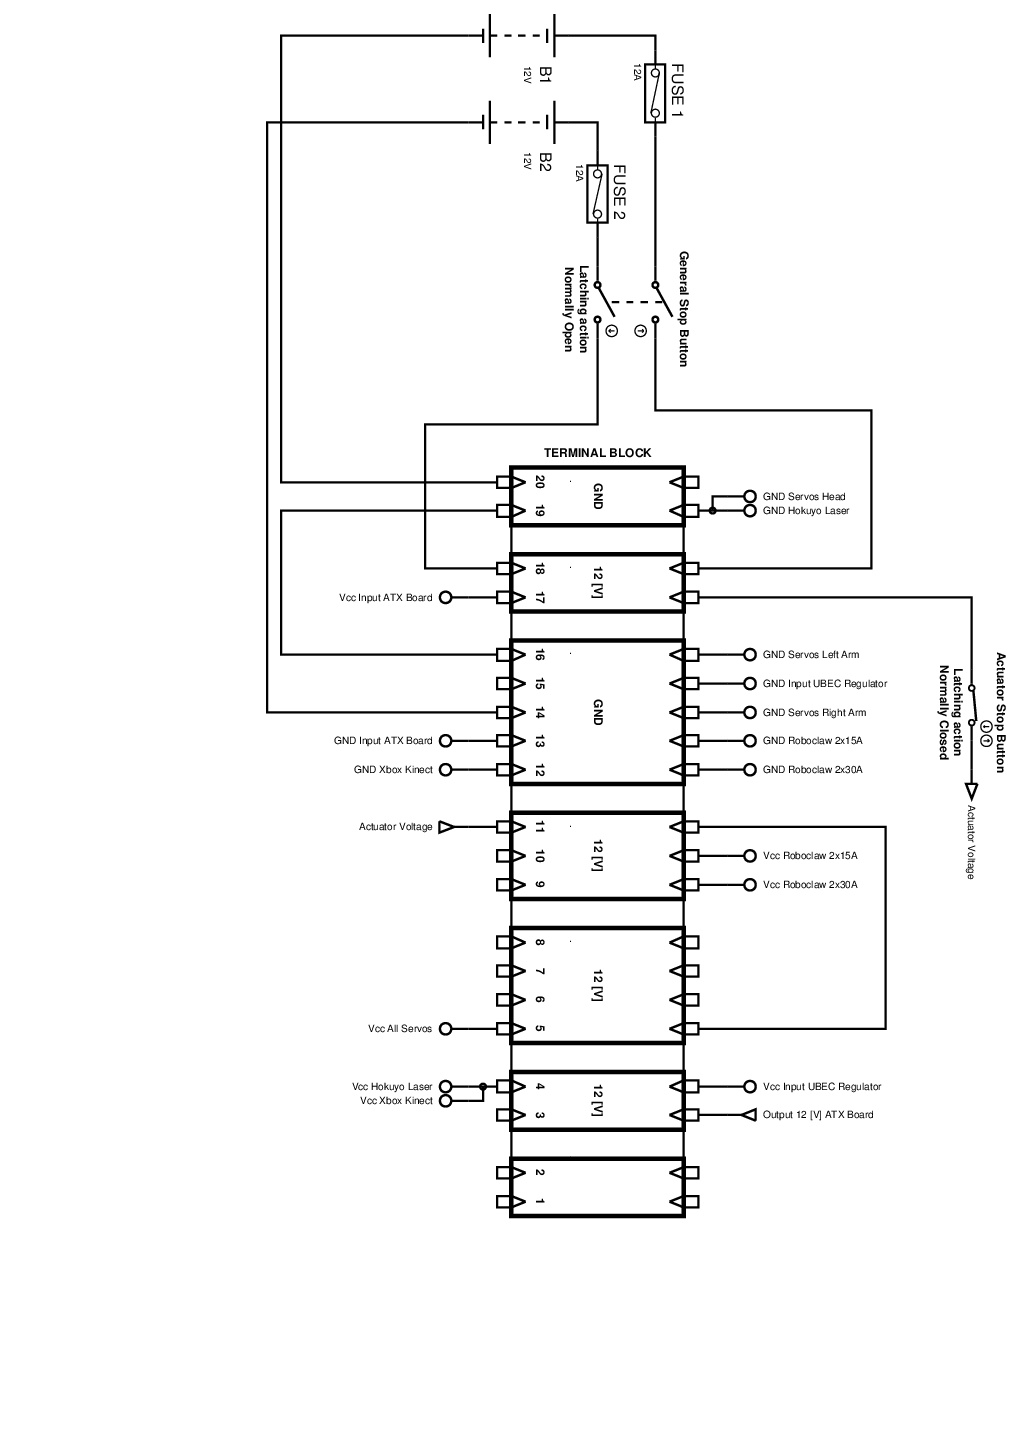
\includegraphics[width=1.1\textwidth]{Figures/Hardware/Esquematicos/JustinaWiringDiagram.jpg}
\captionof{figure}{Diagrama general}
\label{fig:Hardware:Partes:Diagrama:Esquematico:General}
\end{center}

\subsection{Diagrama esquematico Roboclaws}

%Figura
\begin{center}
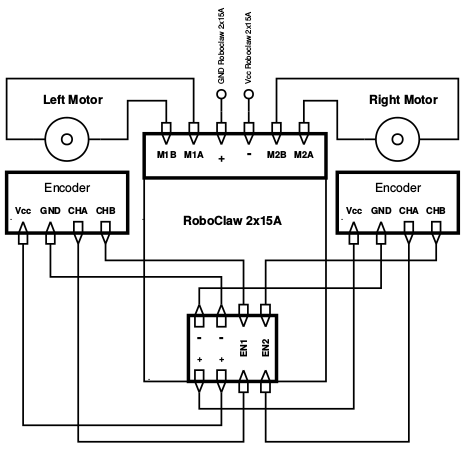
\includegraphics[width=0.75\textwidth]{Figures/Hardware/Esquematicos/Roboclaw_1.png}
\captionof{figure}{Diagrama de la roboclaw 2x15A}
\label{fig:Hardware:Partes:Diagrama:Esquematico:Roboclaw:1}
\end{center}

%Figura
\begin{center}
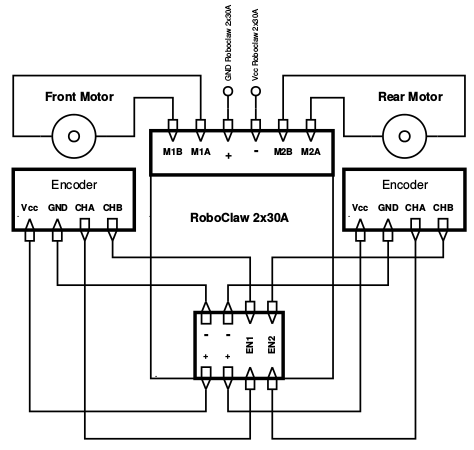
\includegraphics[width=0.75\textwidth]{Figures/Hardware/Esquematicos/Roboclaw_2.png}
\captionof{figure}{Diagrama de la roboclaw 2x30A}
\label{fig:Hardware:Partes:Diagrama:Esquematico:Roboclaw:2}
\end{center}



\chapter{Diseño mecánico}
\chapter{Software}
\chapter{Referencias y ayuda}
\end{document}